\chapter{Implementation}\label{cha:implementation}

This chapter describes the design and implementation of the \emph{QBF Transformer} tool. 
The tool is written in Python~3 and implements the five-step experimental pipeline introduced in Chapter~\ref{cha:introduction}. 
The architecture is organized into five layers, each with a clearly defined responsibility. Figure~\ref{fig:classdiagram} shows the class diagram of the complete system.

\begin{figure}[h]
  \centering
  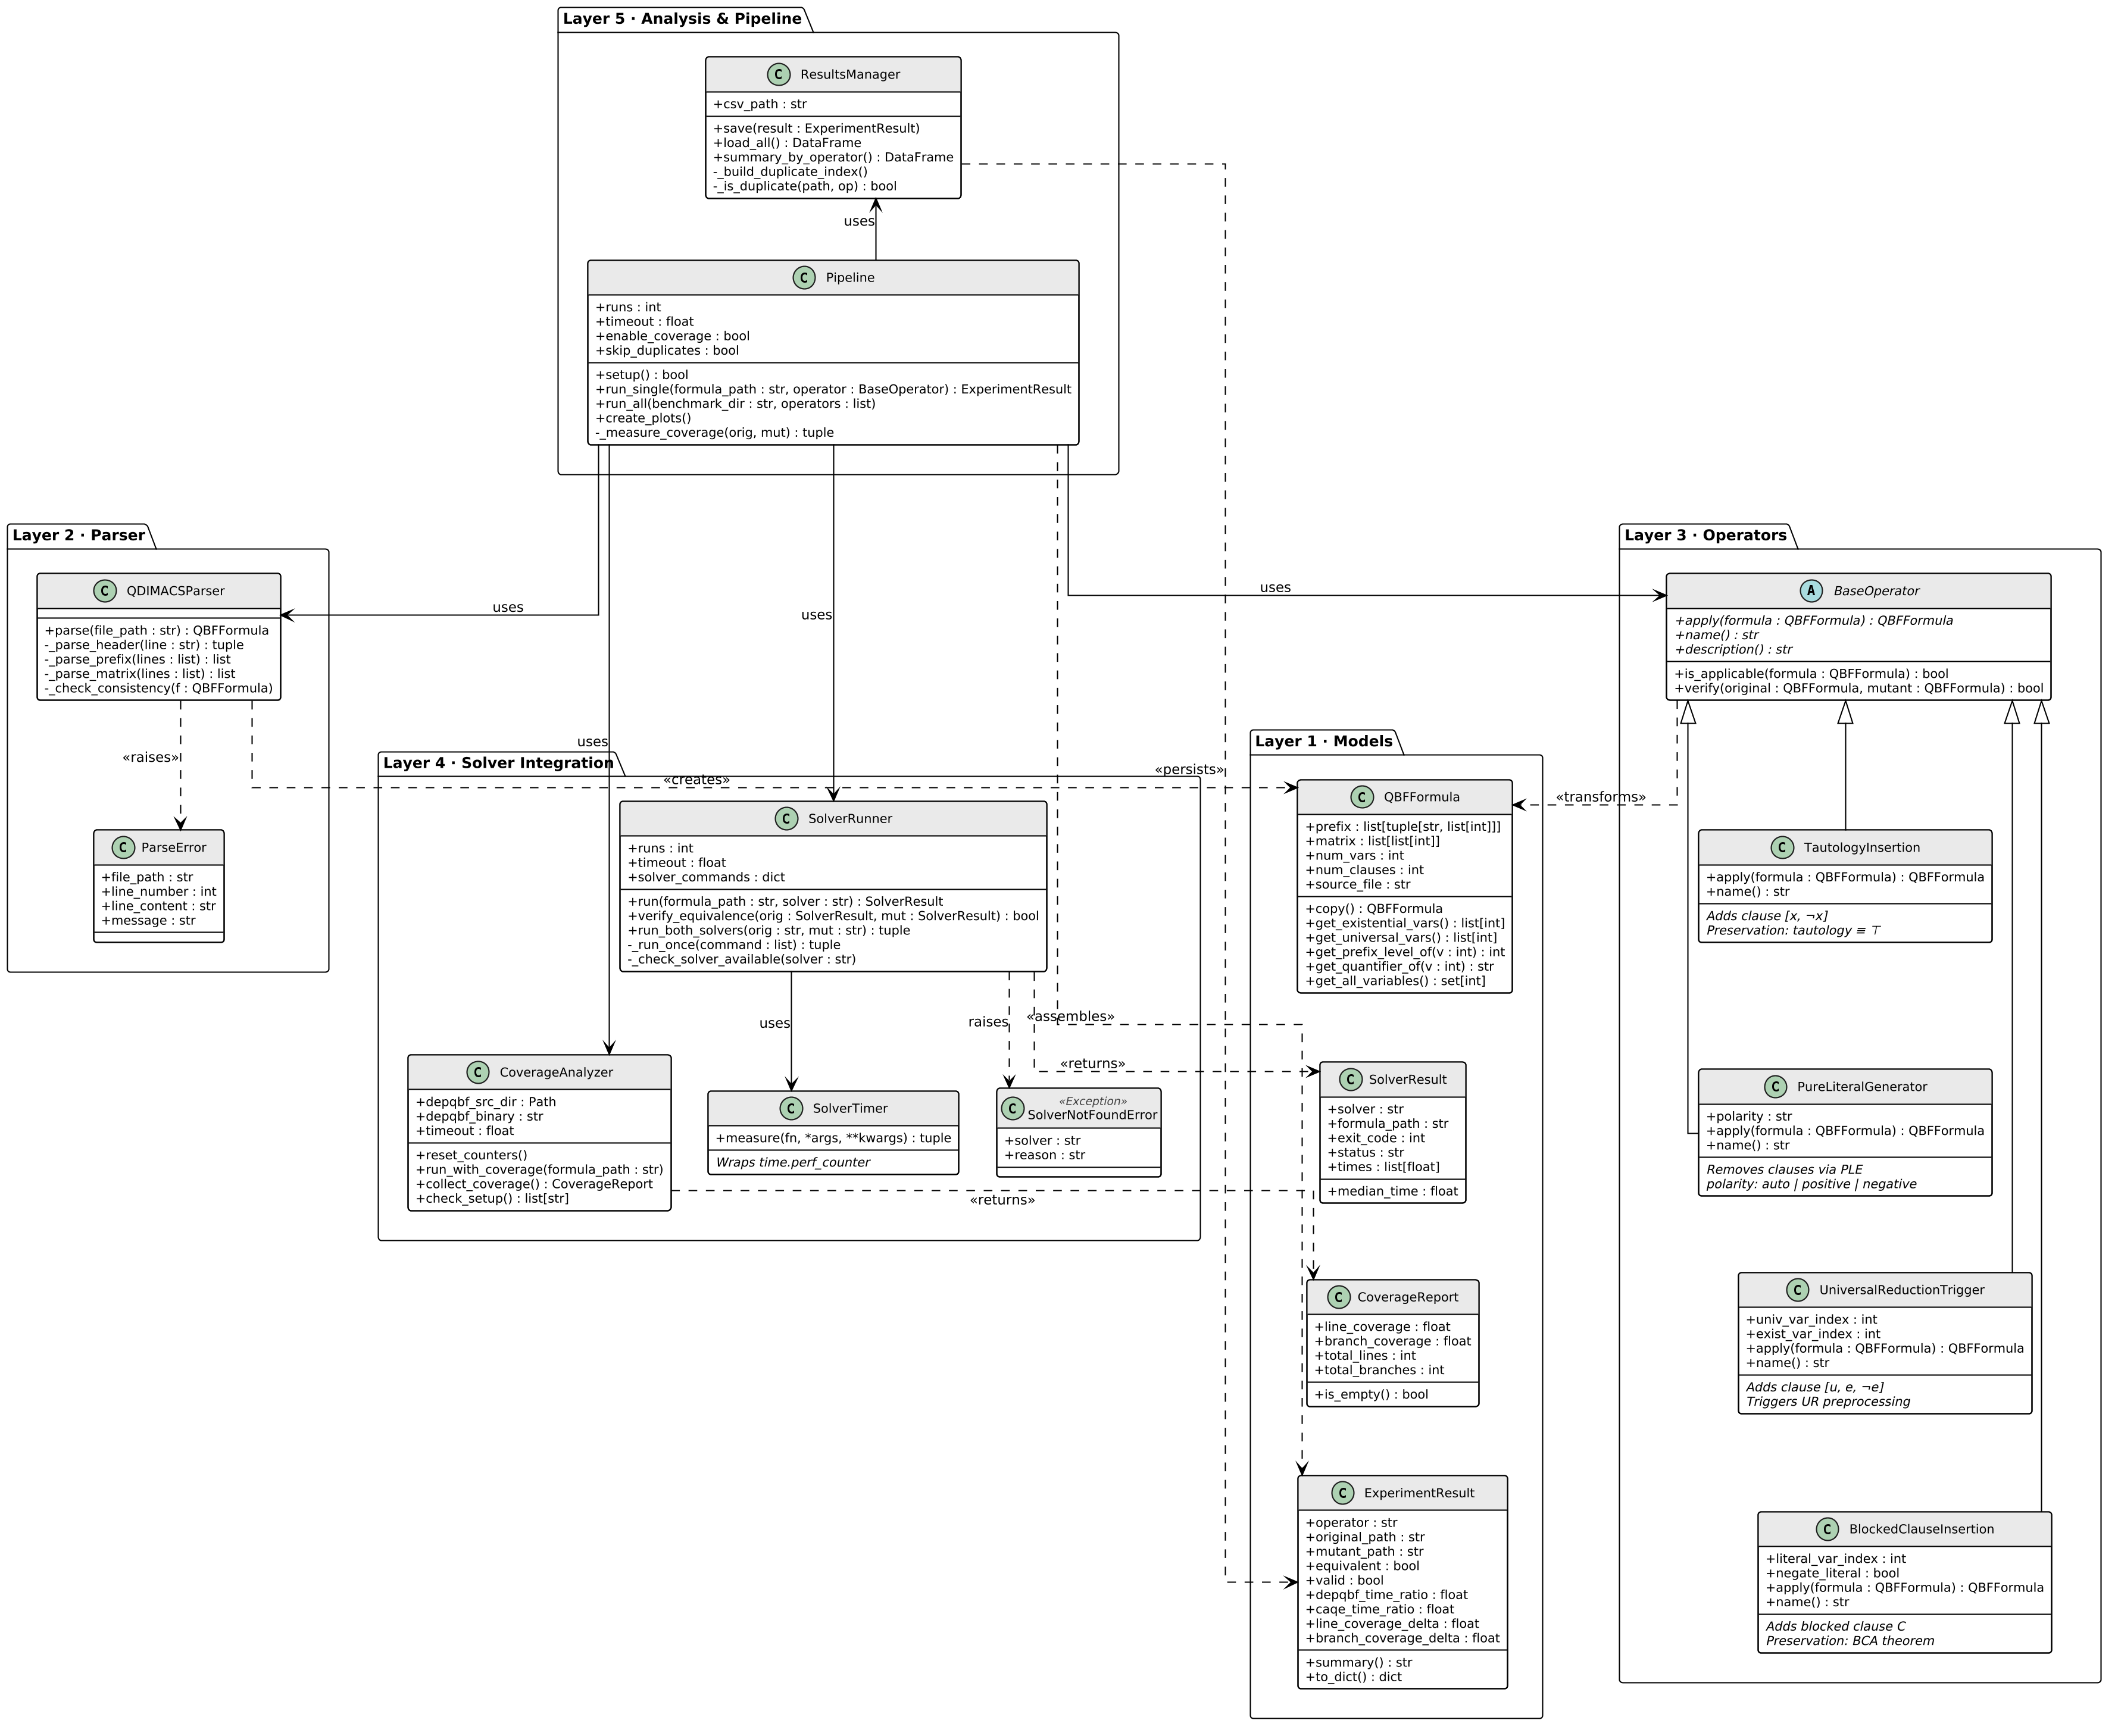
\includegraphics[width=\textwidth]{images/classDiagram.png}
  \caption{Class diagram of the QBF Transformer tool.}
  \label{fig:classdiagram}
\end{figure}

\section{Architecture Overview}\label{sec:architecture}

The system is structured into five layers that correspond directly to the five steps of the experimental pipeline:

\begin{enumerate}
  \item \textbf{Models} --- data classes that represent the domain objects: \texttt{QBFFormula}, \texttt{SolverResult}, \texttt{CoverageReport}, and \texttt{ExperimentResult}.
  \item \textbf{Parser} --- the \texttt{QDIMACSParser} and \texttt{ParseError} classes, which read \texttt{.qdimacs} files and validate their structure.
  \item \textbf{Operators} --- the \texttt{BaseOperator} abstract class and its four concrete subclasses, one per transformation.
  \item \textbf{Solver integration} --- \texttt{SolverTimer}, \texttt{SolverRunner}, and \texttt{CoverageAnalyzer}, which invoke the external solvers and collect measurements.
  \item \textbf{Analysis and pipeline} --- \texttt{ResultsManager}, the \texttt{Pipeline} class in \texttt{main.py}, which orchestrate the full experiment loop and persist results, and a Jupyter notebook(\texttt{\seqsplit{qbf\_solver\_analysis\_notebook.ipynb}}), 
        located in the project root directory, for interactive plot generation and data analysis.

\end{enumerate}

The dependency direction is strictly top-down: each layer uses only 
the layer below it, and no circular dependencies exist between 
modules. An additional utility script, \texttt{filter\_benchmarks.py}, 
is provided outside the main pipeline to select suitable benchmark formulas 
from the QBFLIB repository by filtering on variable count, clause count, 
and prefix-block count; it was used to produce the 50 
benchmark formulas evaluated in Chapter~\ref{cha:evaluation}.

\section{Parser}\label{sec:parser}

The \texttt{QDIMACSParser} class reads a \texttt{.qdimacs} file line by line and constructs a \texttt{QBFFormula} object. Parsing proceeds in four stages:

\begin{enumerate}
  \item \textbf{Comment and blank line removal.} Lines beginning with \texttt{c} and empty lines are discarded. All remaining lines are kept with their original line numbers for error reporting.
  \item \textbf{Header parsing.} The first non-comment line must match the pattern \texttt{p cnf <num\_vars> <num\_clauses>}. Both integers are validated to be positive.
  \item \textbf{Prefix parsing.} Consecutive lines beginning with \texttt{a} (universal) or \texttt{e} (existential) are parsed into a list of \texttt{(quantifier, variables)} tuples. Each line must be terminated by \texttt{0}.
  \item \textbf{Matrix parsing.} The remaining lines are parsed as clauses. Each clause is a list of non-zero signed integers terminated by \texttt{0}.
\end{enumerate}

After parsing, a consistency check verifies that the number of parsed clauses matches \texttt{num\_clauses} from the header, and that every variable referenced in the matrix appears in the prefix. Any violation raises a \texttt{ParseError} that includes the file path, line number, and offending line content, enabling precise diagnosis.

\section{Operator Design}\label{sec:operators-impl}

All four transformation operators share a common interface defined by the abstract base class \texttt{BaseOperator}. The class enforces the \emph{Template Method} pattern: subclasses must implement three abstract methods and may override two optional ones.

\begin{description}
  \item[\texttt{apply(formula)}] Applies the transformation and returns a new \texttt{QBFFormula} object. The original formula must never be modified; the method always calls \texttt{formula.copy()} before making any changes.
  \item[\texttt{name()}] Returns a unique, machine-readable identifier string (e.g.\ \texttt{"tautology\_insertion"}), used as a column value in the CSV output and as a file-name suffix for mutants.
  \item[\texttt{description()}] Returns a human-readable explanation of the transformation.
  \item[\texttt{is\_applicable(formula)}] (optional) Returns \texttt{True} if the preconditions for the operator are met. For example, \texttt{UniversalReductionTrigger} requires at least one universal variable $u$ and one existential variable $e$ with $\mathrm{level}(u) < \mathrm{level}(e)$ (see Section~\ref{sec:ur}). If \texttt{is\_applicable} returns \texttt{False}, the pipeline skips the experiment rather than raising an error.
  \item[\texttt{verify(original, mutant)}] (optional) Performs a post-hoc structural sanity check. This is not a full equivalence proof --- that role is played by the solvers --- but a fast check that the transformation was carried out as intended (e.g.\ the mutant has exactly one more clause than the original).
\end{description}

The eight operator instances registered in \texttt{main.py} are:

\begin{itemize}
  \item \texttt{TautologyInsertion()}
  \item 
    \texttt{\seqsplit{PureLiteralGenerator(polarity="auto")}}, 
    \texttt{\seqsplit{PureLiteralGenerator(polarity="positive")}}, 
    \texttt{\seqsplit{PureLiteralGenerator(polarity="negative")}}
  \item \texttt{UniversalReductionTrigger()}
  \item \texttt{BlockedClauseInsertion()}, 
    \texttt{BlockedClauseInsertion(negate\_literal=True)}, 
    \texttt{BlockedClauseInsertion(literal\_var\_index=1)}
\end{itemize}


Each variant has a distinct \texttt{name()} return value, ensuring that 
results from different configurations of the same operator are stored as 
separate rows in the CSV. 
For \texttt{BlockedClauseInsertion}, the suffix \texttt{\_neg} is appended when 
\texttt{negate\_literal=True}, and the suffix \texttt{\_v\{index\}} is appended when \texttt{literal\_var\_index} 
is non-zero; thus \texttt{\seqsplit{BlockedClauseInsertion(literal\_var\_index=1)}} 
produces the name \texttt{blocked\_clause\_insertion\_v1}.

\section{Solver Integration}\label{sec:solver-impl}

\subsection{SolverTimer and SolverRunner}

Runtime measurement is handled by \texttt{SolverTimer}, which wraps each solver invocation with \texttt{time.perf\_counter}. This clock is monotonic and unaffected by system time corrections, making it suitable for high-resolution process timing.

\texttt{SolverRunner} invokes the external solver binaries via Python's \texttt{subprocess} module. Each solver is called with the path to the formula file as a command-line argument:

\begin{listing}[H]
\caption{Solver invocation commands.}
\label{lst:solver-calls}
\begin{minted}[frame=single,fontsize=\small]{text}
# DepQBF
depqbf --qdo <formula.qdimacs>

# CAQE
caqe <formula.qdimacs>
\end{minted}
\end{listing}

The solver's exit code is interpreted according to the QDIMACS convention: 
exit code \texttt{10} maps to \texttt{SAT}, exit code \texttt{20} maps to 
\texttt{UNSAT}, and any other exit code (including timeout) is recorded as 
\texttt{ERROR}. Each formula is solved once per experiment. Since the primary 
research focus is on correctness (equivalence preservation) and code coverage 
rather than on precise performance benchmarking, a single run is sufficient to 
detect operator-specific differences in solver behavior. The reported runtime 
is the wall-clock time of that run.

The \emph{runtime ratio} for a single experiment is defined as:
\[
  \text{ratio} = \frac{\text{time}(\text{mutant})}{\text{time}(\text{original})}.
\]
A ratio greater than $1.0$ indicates that the mutant takes longer to solve; a ratio less than $1.0$ indicates that the mutant is solved faster.

\subsection{Equivalence Verification}\label{sec:equivalence-verification-impl}

After both the original and the mutant have been solved, 
\texttt{SolverRunner} checks that the results are consistent. 
An experiment is marked \texttt{equivalent = True} if and only 
if the status of the original and the status of the mutant are 
identical (both SAT or both UNSAT) for \textbf{DepQBF}. The CAQE 
results are recorded in the CSV and can be inspected post-hoc, 
but are not used as part of the formal equivalence flag. Any 
discrepancy in the DepQBF results is flagged as a truth-value 
violation and excluded from the runtime and coverage analysis.

\section{Coverage Analysis}\label{sec:coverage-impl}

Code coverage is measured using \texttt{gcov}, which requires DepQBF to be compiled with GCC instrumentation flags:

\begin{listing}[H]
\caption{DepQBF instrumented build command.}
\label{lst:gcov-build}
\begin{minted}[frame=single,fontsize=\small]{bash}
make CFLAGS="-fprofile-arcs -ftest-coverage -O0"
\end{minted}
\end{listing}

The \texttt{CoverageAnalyzer} class implements a three-step measurement protocol for each formula:

\begin{enumerate}
  \item \textbf{Reset.} All \texttt{.gcda} files in the DepQBF source directory are deleted. This clears the execution counters from any previous run.
  \item \textbf{Execute.} DepQBF is invoked once on the formula via \texttt{subprocess}. The instrumented binary writes \texttt{.gcda} files recording which basic blocks were executed and how many times.
  \item \textbf{Collect.} \texttt{gcov} is called on the DepQBF source files. Its standard output contains lines of the form \texttt{Lines executed: X\% of N} and \texttt{Branches executed: Y\% of M}, which are extracted by the \texttt{CoverageAnalyzer} parser and stored in a \texttt{CoverageReport} object.
\end{enumerate}

This protocol is executed twice per experiment: once for the original formula and once for the mutant. The coverage delta is then computed as:
\[
  \Delta_{\text{line}} = \text{line\_coverage}(\text{mutant}) - \text{line\_coverage}(\text{original}),
\]
and analogously for branch coverage. A positive delta indicates that the mutant caused the solver to traverse additional code paths.

\textbf{Platform note.} On macOS, Apple Clang does not support \texttt{gcov} instrumentation. The instrumented DepQBF binary must therefore be compiled with \texttt{gcc-15} installed via Homebrew, and the \texttt{gcov} binary must be explicitly set to \texttt{gcov-15}.

\section{Pipeline and Result Persistence}\label{sec:pipeline-impl}

The \texttt{Pipeline} class in \texttt{main.py} orchestrates the complete experimental loop. Its \texttt{run\_all()} method iterates over every combination of benchmark formula and operator, calling \texttt{run\_single()} for each pair. The \texttt{run\_single()} method executes the five pipeline steps in sequence:

\begin{enumerate}
  \item Parse the original formula with \texttt{QDIMACSParser}.
  \item Apply the operator to produce a mutant and write it to disk as a \texttt{.qdimacs} file.
  \item Run both solvers on original and mutant with \texttt{SolverRunner}.
  \item Measure coverage for both with \texttt{CoverageAnalyzer}.
  \item Assemble an \texttt{ExperimentResult} and persist it via \texttt{ResultsManager}.
\end{enumerate}

\texttt{ResultsManager} appends each result immediately to a CSV file using \texttt{pandas}. 
All plots and statistical summaries are produced separately in the Jupyter notebook \texttt{qbf\_solver\_analysis\_\allowbreak notebook.ipynb}, which loads the CSV and generates the figures used in Chapter~\ref{cha:evaluation}. 
Writing incrementally rather than in batch ensures that no data is lost if the pipeline is interrupted. 
A duplicate detection mechanism based on an in-memory set (keyed on formula path, operator name, and mutant path) prevents re-running experiments that are already present in the CSV, enabling the pipeline to be resumed after interruption in $O(1)$ per lookup.

The CSV schema contains one row per experiment with the following columns: \texttt{operator}, \texttt{original\_path}, \texttt{mutant\_path}, \texttt{equivalent}, \texttt{valid}, solver status and median time 
for both solvers on both formulas, the runtime ratio for each solver, and line and branch coverage for original, mutant, and their delta. This flat structure is directly consumed by the Jupyter notebook described in Chapter~\ref{cha:evaluation}.

\section{Command-Line Interface}\label{sec:cli}

The tool is invoked from the command line via \texttt{main.py}. The most common usage patterns are:

\begin{listing}[H]
\caption{CLI usage examples.}
\label{lst:cli}
\begin{minted}[frame=single,fontsize=\small]{bash}
# Run all formulas x all operators
python main.py

# Run one specific formula
python main.py --formula benchmarks/formula_001.qdimacs

# Run one specific operator only
python main.py --operator tautology_insertion

# Adjust run count and timeout
python main.py --timeout 30

# Disable coverage measurement (faster)
python main.py --no-coverage

# Generate summary from existing CSV (no new experiments)
python main.py --plots-only
\end{minted}
\end{listing}

Additional configuration arguments control solver binary paths 
(\texttt{--depqbf-src}, \texttt{--depqbf-binary}), the output 
CSV path (\texttt{--results-csv}), the benchmark directory 
(\texttt{--benchmark-dir}), and duplicate detection behaviour (\texttt{--no-skip-duplicates}, which disables the duplicate check and forces re-running all experiments). 
By default, the pipeline skips formula--operator combinations that are already present in the 
CSV, enabling interrupted runs to be resumed without recomputing 
existing results.

%%% Local Variables:
%%% tex-command: "pdflatex"
%%% TeX-master: "../main"
%%% TeX-command-extra-options: "-shell-escape"
%%% End: